\chapter{Build and understand dataset}
First and foremost, we have to build a coherent dataset (by cross-referencing sources) to be able to train the models depending on what information are available and how do we want to use it. A wealth of data is available on the "SNCF" and "INSEE" websites: the company and the organization make available a vast amount of open data \url{https://ressources.data.sncf.com}, \url{https://statistiques-locales.insee.fr/}.

\section{Build dataset}
Deliverable of this chapter: The built dataset (before preprocessing) is available on on GitHub:
\begin{center}
    \url{https://github.com/pierre-jezegou/fib-ml-project/releases/download/build-dataset-1.0.3/dataset.csv}
\end{center}
This construction allows us to have enough data (especially features), from two different and independent sources, to obtain an analysis as close as possible to reality. All the raw csv files are stored in the \code{data/} folder in the repository.

\subsection{Consolidating City Statistics and Attraction Area Data (INSEE)}
In \href{https://github.com/pierre-jezegou/fib-ml-project/blob/main/consolidate_cities.py}{\code{consolidate_cities.py}} the process of consolidating city statistics and attraction area data is described. This involves loading, cleaning, merging, aggregating, translating column names, and exporting the consolidated dataset.

The process starts by loading two datasets from INSEE institute, \code{cities_statistics.csv} and \code{attraction_area_per_city.csv}, containing city statistics and information on attraction areas, respectively. After merging the datasets based on \code{city_code}, the numeric data is aggregated per \code{Aire d'attraction des villes 2020} to obtain summarized statistics for each attraction area. Column names are translated to English for clarity and consistency, and the consolidated dataset is exported as \code{consolidated-cities.csv} for further analysis.

\subsection{Building Train Station Dataset (SNCF) - Final dataset}
Then, the process of constructing a dataset related to train stations is done in several steps of data transformation, merging, and integration with cities information.

\subsubsection{Data Transformation}
First, we need to improve columns' data coherence between files: \code{transform_uid} function is defined to format the UIC code into a standardized string format. Then, raw datasets provided by SNCF are processed:
\begin{itemize}
    \item \code{frequentation-gares-raw.csv}: This dataset, representing train station traffic, undergoes transformation where the 'UIC' column is converted to string format and filled to a length of 10 characters with leading zeros. Additionally, the column 'Nom de la gare' is renamed to 'Gare' for clarity.
    \item Other datasets such as services in stations \code{gares-equipees-du-wifi-raw.csv}: be sure to have a clear UIC code to allow merging operations.
\end{itemize}

\subsubsection{Data Merging}
The datasets are then merged using the \code{merge_data_train_stations} function: it iterates through a list of file names, merges datasets based on the 'UIC' column, and performs necessary column operations for clarity.

\subsubsection{Integration with Consolidated Cities}
The resulting train station dataset is then integrated with consolidated cities information. The dataset containing consolidated cities data is loaded, and a merge operation is performed based on the \code{city_code} column. The final merged dataset is saved as \code{dataset.csv}.

\begin{lstlisting}[language=Python]
result = pd.merge(train_stations, consolidated_cities, on="city_code")
\end{lstlisting}

The final columns (features) are describe in the README file in the GitHub repository: \url{https://github.com/pierre-jezegou/fib-ml-project/blob/main/README.md}

\section{Dataset inspection}
\subsection{First inspection}
First, we analyzed the dataset using the \code{dataset.describe()} function from pandas. Our interpretations are as follows:
\begin{itemize}
    \item \textbf{Zero Values}: Some numerical columns, such as \code{total_passengers_2022}, have suspicious zero values needing special handling.
    \item \textbf{High Variability}: Columns like \code{total_passengers_2022} exhibit high standard deviations, indicating significant variability.
    \item \textbf{Missing Data}: Columns such as \code{distr_histoires_courtes} have significantly fewer entries, indicating missing data that may require imputation or removal.
\end{itemize}
Next steps include handling missing values by imputing or removing them, normalizing or standardizing numerical columns for machine learning models, and identifying and handling outliers to ensure robust analysis.\\

We can also have check how many missing values do we have on each variable: \code{dataset.isna().sum()}. For some of the train station related features, there are 7 missing values, but for services provided in stations, there are lot more missing data : 2179. We have to take a decision regarding those two types of missing values.

\subsection{Understand the data}
\begin{figure}[h]
    \centering
    \begin{subfigure}[b]{0.45\textwidth}
         \centering
         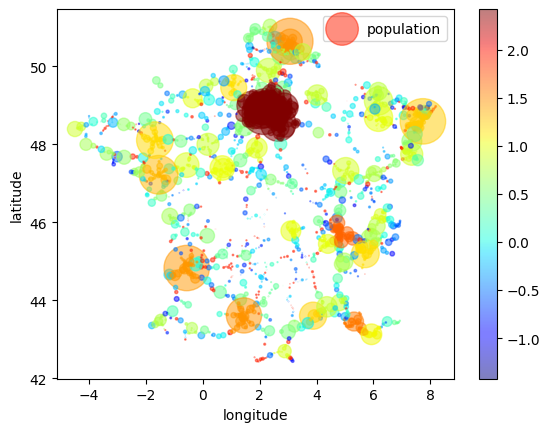
\includegraphics[width=\textwidth]{assets/images/french-map-train-stations.png}
     \end{subfigure}
    \hfill
     \begin{subfigure}[b]{0.4\textwidth}
         \centering
         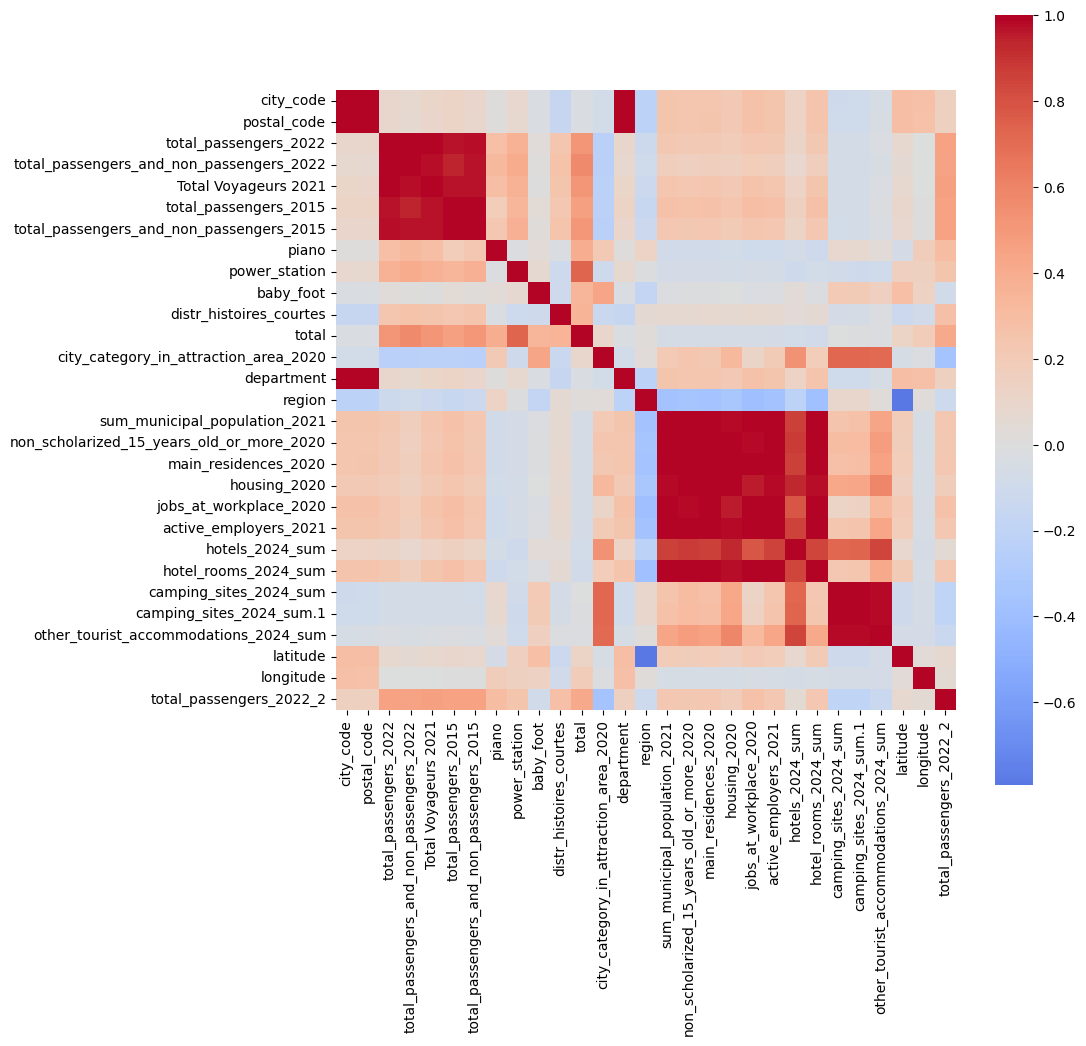
\includegraphics[width=\textwidth]{assets/images/variable-correlation.png}
     \end{subfigure}
     \caption{Examples of data visualizations to understand the dataset}
\end{figure}
Since Paris is the hub for many train lines, we think it can be interesting to compute the distance to Paris. We also observed strong correlations between some variables, so we will remove redundant ones during feature engineering.\label{paris:center-france}